\documentclass{modificopy}
\usepackage{lipsum}

\usepackage{titlesec}
\usepackage{tocloft}
\usepackage{hyperref}
\usepackage{amsmath}
\usepackage{amssymb}

\hypersetup{
    colorlinks=true,
    linkcolor=blue!60!black,
    urlcolor=blue!60!black,
    citecolor=green!40!black
}

\title{SmartClub Analytics}

\begin{document}

%----------- Informations du rapport ---------

\titre{SmartClub Analytics : Plateforme Intelligente \\ pour la Gestion et le Suivi des Clubs de Football}

\sujet{Projet de Fin d'Études \\ Année Académique 2024--2025}

\enseignant{[Nom de l'Encadrant] \\ [Poste]}

\eleves{Bilel \textsc{Amri}}

%----------- Initialisation -------------------

\fairemarges
\fairepagedegarde

\newpage

\chapter*{Remerciements}
\addcontentsline{toc}{chapter}{Remerciements}

Je tiens à exprimer ma profonde gratitude à toutes les personnes qui ont contribué, de près ou de loin, à la réussite de ce projet.

Je remercie chaleureusement mon encadrant, [Nom de l'encadrant], pour sa disponibilité, ses conseils avisés et son accompagnement tout au long de ce travail. Son expertise et ses orientations m'ont permis de mener à bien ce projet dans les meilleures conditions.

Je remercie également l'équipe pédagogique de TEK-UP pour la qualité de la formation dispensée tout au long de mon parcours académique, ainsi que pour leur soutien et leurs encouragements.

Enfin, je souhaite exprimer ma reconnaissance envers ma famille et mes proches pour leur soutien indéfectible et leurs encouragements constants.

\newpage

\chapter*{Résumé}
\addcontentsline{toc}{chapter}{Résumé}

\section*{Français}

\textbf{SmartClub Analytics} est une plateforme complète de gestion sportive, pilotée par l'intelligence artificielle, conçue pour les clubs de football professionnels. Elle intègre la prédiction des risques de blessure, la planification nutritionnelle personnalisée, le scouting intelligent de joueurs, ainsi qu'un assistant conversationnel multimodal — le tout au sein d'un tableau de bord unifié et authentifié.

La plateforme s'appuie sur trois jeux de données réels du monde sportif : SoccerMon (50 joueurs, 731 jours de suivi, 162 blessures), StatsBomb Open Data (Liga Espagnole 2020/21) et USDA FoodData Central (436 aliments de référence). Le cœur de l'intelligence artificielle repose sur deux modèles CatBoost — un classifieur binaire de risque de blessure (AUC 0,896) et un régresseur de durée d'absence (MAE ~21 jours) — entraînés sur ces données authentiques et intégrés via une API REST Django.

L'architecture technique combine un backend Django 4.2 avec Django REST Framework, un frontend React 18 avec Recharts pour la visualisation de données, un chatbot à base de LLM (Groq/OpenAI) avec support multilingue (EN/FR/AR/TN), et un système de monitoring temps réel des performances API. L'authentification est assurée par JWT avec un contrôle d'accès basé sur les rôles (RBAC) à cinq niveaux.

\vspace{0.5cm}
\textbf{Mots-clés :} Intelligence Artificielle, Sport, Prédiction de Blessure, Machine Learning, CatBoost, Django, React, Nutrition, Scouting, Chatbot LLM.

\section*{English}

\textbf{SmartClub Analytics} is a comprehensive AI-driven sports management platform designed for professional football clubs. It integrates injury risk prediction, personalized nutrition planning, intelligent player scouting, and a multimodal conversational assistant — all within a unified, authenticated dashboard.

The platform relies on three real-world sports datasets: SoccerMon (50 players, 731 days, 162 injuries), StatsBomb Open Data (La Liga 2020/21), and USDA FoodData Central (436 reference foods). The AI core consists of two CatBoost models — a binary injury risk classifier (AUC 0.896) and an absence duration regressor (MAE ~21 days) — trained on these authentic datasets and integrated via a Django REST API.

The technical architecture combines a Django 4.2 backend with Django REST Framework, a React 18 frontend with Recharts for data visualization, an LLM-powered chatbot (Groq/OpenAI) with multilingual support (EN/FR/AR/TN), and a real-time API performance monitoring system. Authentication is ensured by JWT with a five-level role-based access control (RBAC).

\vspace{0.5cm}
\textbf{Keywords:} Artificial Intelligence, Sports, Injury Prediction, Machine Learning, CatBoost, Django, React, Nutrition, Scouting, LLM Chatbot.

\newpage

\chapter*{Introduction générale}
\addcontentsline{toc}{chapter}{Introduction générale}

La transformation numérique du sport professionnel s'est considérablement accélérée au cours des dernières années, faisant de l'analyse de données et de l'intelligence artificielle des leviers stratégiques majeurs pour les clubs de football. Selon un rapport de Deloitte publié en 2024, le marché mondial de l'analyse sportive (Sports Analytics) a dépassé les 4 milliards de dollars, avec un taux de croissance annuel composé de 22\,\%. Les clubs de football professionnels génèrent aujourd'hui des volumes massifs de données — tracking GPS, capteurs physiologiques, données de performance, dossiers médicaux, données nutritionnelles — dont l'exploitation optimale constitue à la fois un défi technique et une opportunité compétitive décisive.

Dans ce contexte, la gestion de la santé des joueurs occupe une place centrale. Les blessures sportives représentent un coût économique considérable pour les clubs : selon une étude publiée dans le British Journal of Sports Medicine, un club de football professionnel européen de première division subit en moyenne 15 à 20 blessures par saison, entraînant un coût salarial direct estimé entre 15 et 30 millions d'euros par an pour les clubs de l'élite. Au-delà de l'aspect financier, l'impact sur les performances sportives et la compétitivité de l'équipe est tout aussi significatif.

Parallèlement, la nutrition sportive personnalisée émerge comme un facteur différenciant majeur dans l'optimisation des performances et la prévention des blessures. Les avancées récentes en science nutritionnelle permettent d'élaborer des plans alimentaires adaptés aux besoins spécifiques de chaque athlète, en fonction de sa position, de son intensité d'entraînement et de son métabolisme individuel.

C'est dans cette perspective que s'inscrit le projet \textbf{SmartClub Analytics}, présenté dans ce mémoire. SmartClub Analytics est une plateforme full-stack intégrant cinq modules complémentaires :

\begin{itemize}
    \item \textbf{PhysioAI v2} : un système de prédiction des risques de blessure basé sur l'apprentissage automatique (CatBoost), intégrant des données de charge d'entraînement, de bien-être subjectif et d'historique médical ;
    \item \textbf{NutriAI} : un module de planification nutritionnelle personnalisée exploitant la base de données USDA FoodData Central (436 aliments) et des règles nutritionnelles adaptées au contexte sportif ;
    \item \textbf{ScoutAI} : un outil de gestion des profils joueurs et des contrats, enrichi par les données StatsBomb de la Liga espagnole ;
    \item \textbf{Chatbot \& Chat LLM} : un assistant conversationnel dual — un chatbot à base de règles (14 intentions) et un agent LLM avec streaming SSE supportant quatre langues (français, anglais, arabe, dialecte tunisien) ;
    \item \textbf{Monitoring} : un tableau de bord temps réel des performances API, de la latence et des ressources système.
\end{itemize}

Le présent rapport s'articule en quatre chapitres complémentaires. Le \textbf{premier chapitre} introduit le contexte général du projet, formalise la problématique et expose les objectifs visés. Le \textbf{deuxième chapitre} dresse un état de l'art des technologies utilisées et spécifie les besoins fonctionnels et non fonctionnels. Le \textbf{troisième chapitre} décrit la conception détaillée de l'architecture, des modèles de données et des algorithmes d'intelligence artificielle. Le \textbf{quatrième chapitre} couvre l'implémentation, les tests et les résultats expérimentaux obtenus. Enfin, une conclusion générale synthétise les contributions du projet et trace les perspectives d'évolution.

\newpage
\tableofcontents

%------------ Corps du rapport ----------------
\chapter{Présentation Générale du Projet}

\section{Introduction}

L'évolution rapide des technologies numériques et de l'intelligence artificielle a profondément transformé le monde du sport professionnel au cours de la dernière décennie. Les clubs de football, en particulier, sont devenus des organisations data-driven où chaque aspect de la performance — de la condition physique des joueurs à la stratégie tactique en passant par la nutrition et la récupération — est désormais mesuré, analysé et optimisé.

La gestion de la santé des joueurs constitue l'un des enjeux les plus critiques pour les clubs modernes. Les blessures sportives représentent non seulement un coût économique direct (salaires versés aux joueurs indisponibles) mais aussi un coût indirect lié à la dégradation des performances collectives. Les statistiques publiées par l'UEFA en 2024 indiquent que les clubs européens de première division enregistrent en moyenne 1,2 blessure par match, avec une indisponibilité moyenne de 18 jours par blessure. Ces chiffres soulignent l'urgence de développer des outils prédictifs et préventifs performants.

C'est dans ce contexte que s'inscrit le projet \textbf{SmartClub Analytics}, dont ce chapitre introductif présente le contexte, la problématique, les objectifs et la vision d'ensemble.

\section{Contexte du projet}

\subsection{La data science au service du football moderne}

Le football professionnel a connu une véritable révolution data au cours des dix dernières années. L'adoption massive des technologies de tracking GPS, des capteurs physiologiques portables et des plateformes d'analyse vidéo a généré un volume de données sans précédent. Selon une étude de McKinsey \& Company (2024), un club de football européen de haut niveau produit aujourd'hui en moyenne plus de 500~Go de données par saison, couvrant :

\begin{itemize}
    \item les \textbf{données de charge d'entraînement} : distance parcourue, accélérations, décélérations, fréquence cardiaque, puissance mécanique ;
    \item les \textbf{données de bien-être subjectif} : qualité du sommeil, fatigue perçue, courbatures, stress, humeur ;
    \item les \textbf{données médicales} : historique des blessures, examens cliniques, imagerie médicale ;
    \item les \textbf{données nutritionnelles} : apports caloriques, macronutriments, compléments alimentaires ;
    \item les \textbf{données de performance en match} : positions, passes, tirs, dribbles, duels.
\end{itemize}

Cependant, la collecte de ces données ne constitue qu'une première étape. Le véritable défi réside dans leur intégration, leur analyse et leur transformation en informations actionnables pour les staffs techniques et médicaux. C'est précisément l'objectif que se fixe SmartClub Analytics.

\subsection{Les datasets fondateurs du projet}

SmartClub Analytics repose sur trois jeux de données réels, soigneusement sélectionnés pour leur qualité scientifique et leur pertinence opérationnelle :

\subsubsection{SoccerMon — Suivi de charge et blessures}

Le dataset \textbf{SoccerMon} \cite{soccermon} constitue la pierre angulaire du module PhysioAI. Il contient les données longitudinales de 50 joueurs de football professionnels suivis sur une période de 731 jours. Le jeu de données inclut :

\begin{itemize}
    \item 19 fichiers de charge d'entraînement et de bien-être (fatigue, qualité du sommeil, courbatures, stress, humeur, charge aiguë/chronique — ACWR) ;
    \item 162 épisodes de blessure documentés avec leur typologie et leur durée ;
    \item Des données quotidiennes de charge d'entraînement (charge aiguë, charge chronique, ratio ACWR, monotonie, strain).
\end{itemize}

Ce dataset, publié dans le cadre de recherches académiques en science du sport, offre une base solide pour l'entraînement de modèles prédictifs de risque de blessure.

\subsubsection{StatsBomb Open Data — Performance en match}

Le dataset \textbf{StatsBomb Open Data} \cite{statsbomb} fournit des données événementielles détaillées de la Liga espagnole 2020/21. Il contient des informations granulaires sur chaque action de jeu : passes, tirs, dribbles, duels, fautes, etc. Ces données enrichissent le module ScoutAI en offrant une évaluation quantitative des performances des joueurs en situation de match.

\subsubsection{USDA FoodData Central — Base nutritionnelle}

La base de données \textbf{USDA FoodData Central} \cite{usdafooddata} constitue la référence mondiale en matière de composition nutritionnelle des aliments. Nous exploitons spécifiquement le sous-ensemble \textit{Foundation Foods}, qui contient 436 aliments de base avec leurs profils nutritionnels complets (calories, protéines, lipides, glucides, fibres, vitamines, minéraux). Cette base alimente le module NutriAI pour la génération de plans nutritionnels personnalisés.

\subsection{L'écosystème technologique}

Le projet s'inscrit dans un écosystème technologique moderne, combinant les meilleures pratiques du développement web full-stack et de l'apprentissage automatique :

\begin{itemize}
    \item \textbf{Python / Django 4.2} pour le backend, offrant un framework mature, sécurisé et extensible ;
    \item \textbf{React 18} pour le frontend, garantissant une expérience utilisateur réactive et moderne ;
    \item \textbf{CatBoost} pour l'apprentissage automatique, choisi pour sa gestion native des caractéristiques catégorielles et sa robustesse ;
    \item \textbf{Groq / OpenAI} pour l'inférence LLM, offrant des performances de pointe en temps réel.
\end{itemize}

\section{Problématique}

\subsection{Énoncé du problème}

La problématique centrale traitée par le projet SmartClub Analytics peut être formulée comme suit :

\begin{quote}
\textit{Comment concevoir et réaliser une plateforme intégrée, exploitant l'intelligence artificielle et l'analyse de données, permettant aux clubs de football professionnels de prédire et prévenir les blessures, d'optimiser la nutrition des joueurs, et de faciliter l'exploration intelligente des données club via le langage naturel ?}
\end{quote}

Cette question soulève plusieurs sous-problèmes techniques et scientifiques :

\begin{itemize}
    \item Comment entraîner un modèle de machine learning capable de prédire le risque de blessure à partir de données longitudinales de charge et de bien-être, avec une précision suffisante pour être cliniquement utile ?
    \item Comment concevoir un système de planification nutritionnelle automatisée, adapté aux besoins spécifiques de chaque joueur (position, intensité d'entraînement, objectifs) ?
    \item Comment intégrer un assistant conversationnel intelligent, capable de comprendre et répondre à des requêtes complexes en langage naturel, dans plusieurs langues, et d'interagir avec l'ensemble des données de la plateforme ?
    \item Comment assurer la sécurité, la confidentialité et le contrôle d'accès aux données sensibles des joueurs (médicales, contractuelles) ?
\end{itemize}

\subsection{Verrous technologiques}

L'analyse préliminaire du projet a mis en évidence plusieurs verrous technologiques :

\begin{enumerate}
    \item \textbf{Verrou des données} : la rareté et la sensibilité des données médicales sportives imposent une stratégie de collecte et d'annotation rigoureuse ;
    \item \textbf{Verrou du déséquilibre de classes} : les épisodes de blessure sont rares par rapport aux jours sans blessure, ce qui impose des techniques spécifiques (oversampling, pondération) ;
    \item \textbf{Verrou de l'interprétabilité} : les prédictions d'un modèle de blessure doivent être explicables pour gagner la confiance des staffs médicaux (besoin d'explicabilité SHAP) ;
    \item \textbf{Verrou multilingue} : le support du dialecte tunisien (arabe dialectal) pour l'assistant conversationnel pose des défis de tokenisation et de compréhension spécifiques.
\end{enumerate}

\section{Objectifs du projet}

\subsection{Objectif principal}

L'objectif principal du projet SmartClub Analytics est de \textbf{concevoir, implémenter et valider une plateforme intégrée de gestion sportive intelligente}, combinant prédiction de blessure, nutrition personnalisée, scouting et interaction en langage naturel.

\subsection{Objectifs spécifiques}

Cet objectif se décline en objectifs spécifiques mesurables :

\begin{itemize}
    \item \textbf{O1 -- PhysioAI} : développer un modèle de prédiction de risque de blessure basé sur CatBoost avec une AUC cible $\geq$ 0,85 ;
    \item \textbf{O2 -- NutriAI} : implémenter un moteur de planification nutritionnelle basé sur règles, couvrant 5 profils d'intensité d'entraînement (repos, léger, modéré, intense, match) ;
    \item \textbf{O3 -- ScoutAI} : réaliser une interface de gestion des profils joueurs et des contrats avec filtres dynamiques ;
    \item \textbf{O4 -- Chatbot} : développer un chatbot à base de règles couvrant 14 intentions métier et un agent LLM supportant 4 langues ;
    \item \textbf{O5 -- Monitoring} : déployer un tableau de bord temps réel des performances API et des ressources système ;
    \item \textbf{O6 -- Sécurité} : implémenter une authentification JWT avec RBAC à 5 niveaux.
\end{itemize}

\section{Vision du projet}

SmartClub Analytics ambitionne de devenir la plateforme de référence pour la gestion intelligente des clubs de football. La vision du projet s'articule autour de trois piliers fondamentaux :

\begin{itemize}
    \item \textbf{Prévention} : anticiper les blessures avant qu'elles ne surviennent, grâce à des modèles prédictifs entraînés sur des données réelles ;
    \item \textbf{Personnalisation} : adapter la nutrition et l'entraînement à chaque joueur, en fonction de ses besoins spécifiques et de son état du moment ;
    \item \textbf{Interaction} : offrir une interface naturelle et intuitive — via le langage naturel — pour interagir avec l'ensemble des données club.
\end{itemize}

\section{Architecture conceptuelle du système}

Le système SmartClub Analytics est structuré autour d'une architecture modulaire en trois couches distinctes, illustrée dans la figure~ci-dessous.

\begin{center}
\begin{tikzpicture}[
    every node/.style={font=\scriptsize},
    layer/.style={rectangle, draw, rounded corners=5pt, minimum width=14cm,
                  minimum height=1.8cm, align=center, fill=blue!8, drop shadow},
    component/.style={rectangle, draw=blue!50, fill=blue!15, rounded corners=3pt,
                      minimum width=2.2cm, minimum height=0.7cm, align=center, font=\scriptsize},
    arr/.style={-Stealth, thick, gray!70!black}
]
% Layer 1: Browser
\node[layer, fill=green!8, draw=green!50!black] (browser) at (0,4.5) {};
\node[font=\bfseries\small] at (browser.north west) [anchor=north west, xshift=4pt, yshift=-4pt] {Couche Présentation -- React 18 Frontend :3000};
\node[component, fill=green!15, draw=green!60!black] (dash) at (-5.5,4.3) {Dashboard\\Recharts};
\node[component, fill=green!15, draw=green!60!black] (physio) at (-3.0,4.3) {PhysioAI\\v2 UI};
\node[component, fill=green!15, draw=green!60!black] (nutri) at (-0.5,4.3) {NutriAI\\UI};
\node[component, fill=green!15, draw=green!60!black] (scout) at (2.0,4.3) {ScoutAI\\UI};
\node[component, fill=green!15, draw=green!60!black] (chat) at (4.5,4.3) {Chatbot\\LLM UI};
\node[component, fill=green!15, draw=green!60!black] (mon) at (6.8,4.3) {Monitoring\\Temps réel};

% Layer 2: API
\node[layer, fill=orange!10, draw=orange!60!black] (api) at (0,1.5) {};
\node[font=\bfseries\small] at (api.north west) [anchor=north west, xshift=4pt, yshift=-4pt] {Couche API -- Django REST Framework :8000};
\node[component, fill=orange!15, draw=orange!70!black] (auth) at (-6.0,1.4) {/api/auth/\\JWT + RBAC};
\node[component, fill=orange!15, draw=orange!70!black] (v2) at (-3.5,1.4) {/api/v2/physio/\\ML Inference};
\node[component, fill=orange!15, draw=orange!70!black] (nutriapi) at (-0.8,1.4) {/api/nutri/\\Food + Plans};
\node[component, fill=orange!15, draw=orange!70!black] (scoutapi) at (1.8,1.4) {/api/scout/\\Players + Contrats};
\node[component, fill=orange!15, draw=orange!70!black] (chatapi) at (4.2,1.4) {/api/chat*/\\Intent + LLM};
\node[component, fill=orange!15, draw=orange!70!black] (monapi) at (6.5,1.4) {/api/monitoring/\\Métriques};

% Layer 3: Data
\node[layer, fill=red!8, draw=red!50!black] (data) at (0,-1.5) {};
\node[font=\bfseries\small] at (data.north west) [anchor=north west, xshift=4pt, yshift=-4pt] {Couche Données -- Datasets + ML};
\node[component, fill=red!15, draw=red!70!black] (socc) at (-5.5,-1.6) {SoccerMon\\50 players};
\node[component, fill=red!15, draw=red!70!black] (stats) at (-3.0,-1.6) {StatsBomb\\Liga 2020/21};
\node[component, fill=red!15, draw=red!70!black] (usda) at (-0.5,-1.6) {USDA Food\\436 foods};
\node[component, fill=red!15, draw=red!70!black] (model) at (2.5,-1.6) {CatBoost\\Risk + Absence};
\node[component, fill=violet!15, draw=violet!70!black] (llm) at (5.5,-1.6) {Groq / OpenAI\\LLM};

% Arrows
\draw[arr] (browser.south) -- node[right, font=\tiny]{HTTP / JSON / SSE} (api.north);
\draw[arr] (api.south) -- node[right, font=\tiny]{ORM / Inference} (data.north);

\end{tikzpicture}

\vspace{0.2cm}
\small\textit{Architecture en trois couches de la plateforme SmartClub Analytics}
\end{center}

\section{Conclusion}

Ce chapitre introductif a présenté le contexte stratégique et scientifique dans lequel s'inscrit le projet SmartClub Analytics. Nous avons mis en lumière les défis auxquels font face les clubs de football professionnels dans la gestion de la santé et de la performance de leurs joueurs, et motivé l'adoption d'une approche intégrée combinant intelligence artificielle, analyse de données et interaction en langage naturel.

La problématique de recherche a été formalisée, les verrous technologiques identifiés, et les objectifs spécifiques énoncés. L'architecture conceptuelle du système a été présentée à grands traits, posant les fondations pour les chapitres suivants.

Le chapitre~2 approfondira l'état de l'art des technologies mobilisées et formalisera les besoins fonctionnels et non fonctionnels qui guideront la conception détaillée présentée au chapitre~3.

\chapter{État de l'Art et Spécification des Besoins}

\section{Introduction}

L'analyse sportive assistée par l'intelligence artificielle connaît une croissance exponentielle ces dernières années. Ce chapitre explore l'état de l'art des technologies et systèmes existants dans le domaine du sport analytics, avant de définir les besoins spécifiques auxquels notre solution SmartClub Analytics doit répondre.

\section{État de l'Art des Systèmes d'Analyse Sportive}

\subsection{Plateformes Commerciales Existantes}

Le marché du sport analytics est dominé par plusieurs plateformes professionnelles :

\begin{itemize}
    \item \textbf{Catapult Sports} : Système de tracking GPS et analyse de charge d'entraînement utilisé par les équipes professionnelles. Propose des métriques de performance et de risque de blessure, mais reste très coûteux et nécessite un hardware propriétaire.
    
    \item \textbf{Zone7} : Plateforme IA spécialisée dans la prédiction de blessures chez les athlètes. Utilise des modèles de deep learning sur des données biomécaniques et physiologiques. Offre une précision remarquable mais son intégration est complexe et son coût d'abonnement élevé.
    
    \item \textbf{Kinexon} : Solution de tracking en temps réel avec capteurs UWB. Fournit des données de position, vitesse, accélération et charge de travail. Principalement utilisé dans les sports d'équipe professionnels.
    
    \item \textbf{StatsBomb} : Plateforme d'analyse de données de football avec des métriques avancées comme les expected goals (xG) et expected assists (xA). Excellente pour l'analyse de performance mais ne couvre pas la prévention des blessures.
\end{itemize}

\subsection{Limitations des Solutions Existantes}

\begin{itemize}
    \item \textbf{Coût prohibitif} : La plupart des solutions professionnelles nécessitent des budgets importants, les rendant inaccessibles aux clubs amateurs et semi-professionnels.
    \item \textbf{Complexité technique} : L'intégration de ces systèmes requiert une expertise technique que peu de clubs possèdent en interne.
    \item \textbf{Manque de personnalisation} : Ces plateformes sont souvent conçues pour des besoins génériques et ne s'adaptent pas aux spécificités de chaque club.
    \item \textbf{Modules disjoints} : Les clubs doivent souvent utiliser plusieurs solutions distinctes pour la nutrition, la physiothérapie, le scouting et la gestion des contrats.
\end{itemize}

\subsection{Avancées en IA pour le Sport}

\subsubsection{Prédiction de Blessures}

La recherche académique a démontré plusieurs approches prometteuses :

\begin{itemize}
    \item \textbf{Modèles de séries temporelles} : L'utilisation de LSTM (Long Short-Term Memory) sur les données de charge d'entraînement permet de prédire les fenêtres de risque accru de blessure avec une précision de 75-85\% \cite{bienefeld2023}.
    
    \item \textbf{ACWR (Acute:Chronic Workload Ratio)} : Métrique standardisée qui compare la charge de travail aiguë (7 jours) à la charge chronique (28 jours). Un ratio entre 0.8 et 1.3 est considéré optimal, tandis que des valeurs supérieures à 1.5 indiquent un risque significatif de blessure \cite{gabbett2016}.
    
    \item \textbf{Random Forests et Gradient Boosting} : Des études récentes montrent que ces algorithmes d'ensemble atteignent une AUC de 0.82-0.88 pour la classification du risque de blessure en utilisant des caractéristiques combinées de charge, de fatigue, et d'historique médical.
\end{itemize}

\subsubsection{Traitement du Langage Naturel pour le Coaching}

Les LLMs (Large Language Models) comme ceux disponibles via l'API Groq ou OpenAI ouvrent de nouvelles possibilités :

\begin{itemize}
    \item \textbf{Analyse conversationnelle} : Permettre aux entraîneurs d'interroger les données sportives en langage naturel.
    \item \textbf{Génération de rapports} : Production automatisée de rapports d'analyse après chaque match ou session d'entraînement.
    \item \textbf{Support multilingue} : Capacité à interagir dans différentes langues (français, anglais, arabe, tunisien) pour s'adapter aux utilisateurs locaux.
\end{itemize}

\subsubsection{Systèmes de Recommandation Nutritionnelle}

L'intégration de bases de données nutritionnelles (telles que FoodData Central de l'USDA) avec des modèles de planification alimentaire permet de générer des plans nutritionnels personnalisés en fonction des objectifs de performance et de récupération des athlètes.

\section{Analyse des Besoins}

\subsection{Besoins Fonctionnels}

L'analyse des besoins a été réalisée en collaboration avec des entraîneurs, des préparateurs physiques et des gestionnaires de clubs sportifs tunisiens.

\subsubsection{Module de Physiothérapie et Prévention des Blessures}

\begin{itemize}
    \item \textbf{BF-01} : Calcul et visualisation de l'ACWR pour chaque joueur.
    \item \textbf{BF-02} : Détection précoce des joueurs à risque de blessure.
    \item \textbf{BF-03} : Recommandations personnalisées de charge d'entraînement.
    \item \textbf{BF-04} : Tableau de bord quotidien des risques de l'effectif.
    \item \textbf{BF-05} : Suivi de l'évolution temporelle des métriques de performance.
\end{itemize}

\subsubsection{Module Nutritionnel}

\begin{itemize}
    \item \textbf{BN-01} : Consultation d'une base de données alimentaires riche (nutriments, calories, macronutriments).
    \item \textbf{BN-02} : Génération de plans nutritionnels personnalisés selon l'intensité d'entraînement.
    \item \textbf{BN-03} : Calcul automatique des macros pour les repas.
    \item \textbf{BN-04} : Recherche d'aliments et de suppléments sportifs.
\end{itemize}

\subsubsection{Module de Scouting et Analyse de Performance}

\begin{itemize}
    \item \textbf{BS-01} : Exploration et filtrage de profils de joueurs.
    \item \textbf{BS-02} : Analyse comparative des performances (xG, xA, passes décisives).
    \item \textbf{BS-03} : Visualisation des métriques clés par poste.
    \item \textbf{BS-04} : Suivi des statistiques de buts et d'assists.
\end{itemize}

\subsubsection{Module Assistant IA Conversationnel}

\begin{itemize}
    \item \textbf{BA-01} : Interface de chat en langage naturel pour interroger toutes les données.
    \item \textbf{BA-02} : Support multilingue (français, anglais, arabe, dialecte tunisien).
    \item \textbf{BA-03} : Exécution d'outils spécialisés (risque de blessure, nutrition, scouting).
    \item \textbf{BA-04} : Streaming des réponses pour une expérience utilisateur fluide.
\end{itemize}

\subsection{Besoins Non-Fonctionnels}

\begin{itemize}
    \item \textbf{BNF-01 - Performance} : Temps de réponse inférieur à 2 secondes pour les requêtes standards, inférieur à 5 secondes pour les analyses complexes.
    \item \textbf{BNF-02 - Sécurité} : Authentification JWT, contrôle d'accès basé sur les rôles (RBAC), protection CSRF.
    \item \textbf{BNF-03 - Évolutivité} : Architecture modulaire permettant l'ajout de nouveaux modules sans impact sur l'existant.
    \item \textbf{BNF-04 - Disponibilité} : Taux de disponibilité de 99,5\% pour les fonctionnalités critiques.
    \item \textbf{BNF-05 - Portabilité} : Déploiement possible sur site (on-premise) ou dans le cloud.
    \item \textbf{BNF-06 - Maintenabilité} : Code documenté, tests automatisés, architecture en couches.
\end{itemize}

\subsection{Diagramme de Cas d'Utilisation}

\begin{figure}[H]
\centering
\begin{tikzpicture}[
    scale=0.85, transform shape,
    actor/.style={rectangle, draw, minimum width=2cm, minimum height=0.8cm, font=\small, rounded corners, fill=blue!10},
    usecase/.style={ellipse, draw, minimum width=2.5cm, minimum height=0.8cm, font=\small, fill=green!10}
]
% Acteurs
\node[actor] (coach) at (-4,4) {Entraîneur};
\node[actor] (physio) at (-4,1) {Physio};
\node[actor] (manager) at (-4,-2) {Manager};
\node[actor] (admin) at (-4,-4) {Admin};

% Système
\draw[thick] (-1,-5) rectangle (12,6);
\node at (5.5,5.5) {\textbf{SmartClub Analytics}};

% Cas d'utilisation - Physio
\node[usecase] (risk) at (2,3) {Consulter risques\\de blessure};
\node[usecase] (acwr) at (5,3) {Visualiser ACWR};
\node[usecase] (profiles) at (8,3) {Profils joueurs};
\node[usecase] (nutrition) at (2,0) {Plans nutritionnels};
\node[usecase] (food) at (5,0) {Base alimentaire};
\node[usecase] (scout) at (8,0) {Analyse\\scouting};
\node[usecase] (chat) at (5,-2) {Assistant IA\\conversationnel};
\node[usecase] (auth) at (2,-4) {Authentification};
\node[usecase] (adminuc) at (8,-4) {Gestion\\utilisateurs};

% Relations acteurs -> cas
\draw (coach) -- (risk);
\draw (coach) -- (acwr);
\draw (coach) -- (chat);
\draw (physio) -- (risk);
\draw (physio) -- (profiles);
\draw (physio) -- (nutrition);
\draw (manager) -- (scout);
\draw (manager) -- (food);
\draw (manager) -- (nutrition);
\draw (admin) -- (auth);
\draw (admin) -- (adminuc);

% Relations include/extend
\draw[->,dashed] (risk) -- node[above,font=\tiny] {include} (acwr);
\draw[->,dashed] (nutrition) -- node[above,font=\tiny] {include} (food);

\end{tikzpicture}
\caption{Diagramme des cas d'utilisation du système SmartClub Analytics}
\label{fig:usecase}
\end{figure}

\section{Choix Technologiques}

\subsection{Backend : Django REST Framework}

Le choix de Django comme framework backend principal est motivé par :

\begin{itemize}
    \item \textbf{Robustesse et maturité} : Django est un framework éprouvé avec une communauté large et active.
    \item \textbf{ORM puissant} : L'Object-Relational Mapping de Django facilite l'interaction avec la base de données PostgreSQL.
    \item \textbf{Sécurité intégrée} : Protection CSRF, XSS, SQL injection, authentification JWT via SimpleJWT.
    \item \textbf{Django REST Framework} : Création rapide d'APIs RESTful avec sérialisation, validation et documentation automatique.
    \item \textbf{Écosystème riche} : Nombreuses extensions disponibles (caching, background tasks, etc.).
\end{itemize}

\subsection{Frontend : React avec Tailwind CSS}

\begin{itemize}
    \item \textbf{React 18} : Bibliothèque JavaScript moderne pour la création d'interfaces utilisateur réactives.
    \item \textbf{Tailwind CSS} : Framework CSS utilitaire permettant un développement rapide et cohérent.
    \item \textbf{Recharts} : Bibliothèque de visualisation de données pour les graphiques (ACWR, tendances, etc.).
    \item \textbf{Architecture modulaire} : Composants réutilisables et lazy-loading pour des performances optimales.
\end{itemize}

\subsection{Intelligence Artificielle : LLM et Machine Learning}

\begin{itemize}
    \item \textbf{API Groq} : Inférence LLM ultra-rapide pour l'assistant conversationnel (modèle Llama 3.1 8B).
    \item \textbf{Scikit-learn} : Implémentation des modèles de prédiction de blessures (Random Forest, Gradient Boosting).
    \item \textbf{FoodData Central} : Base de données nutritionnelle de l'USDA intégrée pour les recommandations alimentaires.
    \item \textbf{Modèles personnalisés} : Notebooks Jupyter pour l'entraînement de modèles de prédiction d'absence et de risque de blessure.
\end{itemize}

\subsection{Infrastructure : Docker et Conteneurisation}

\begin{itemize}
    \item \textbf{Docker Compose} : Orchestration des services (backend, frontend, base de données).
    \item \textbf{Nginx} : Serveur proxy inverse pour le routage et la gestion des requêtes.
    \item \textbf{PostgreSQL} : Base de données relationnelle robuste et performante.
\end{itemize}

\section{Architecture Globale du Système}

\subsection{Vue d'Ensemble}

L'architecture de SmartClub Analytics suit un modèle en couches :

\begin{figure}[H]
\centering
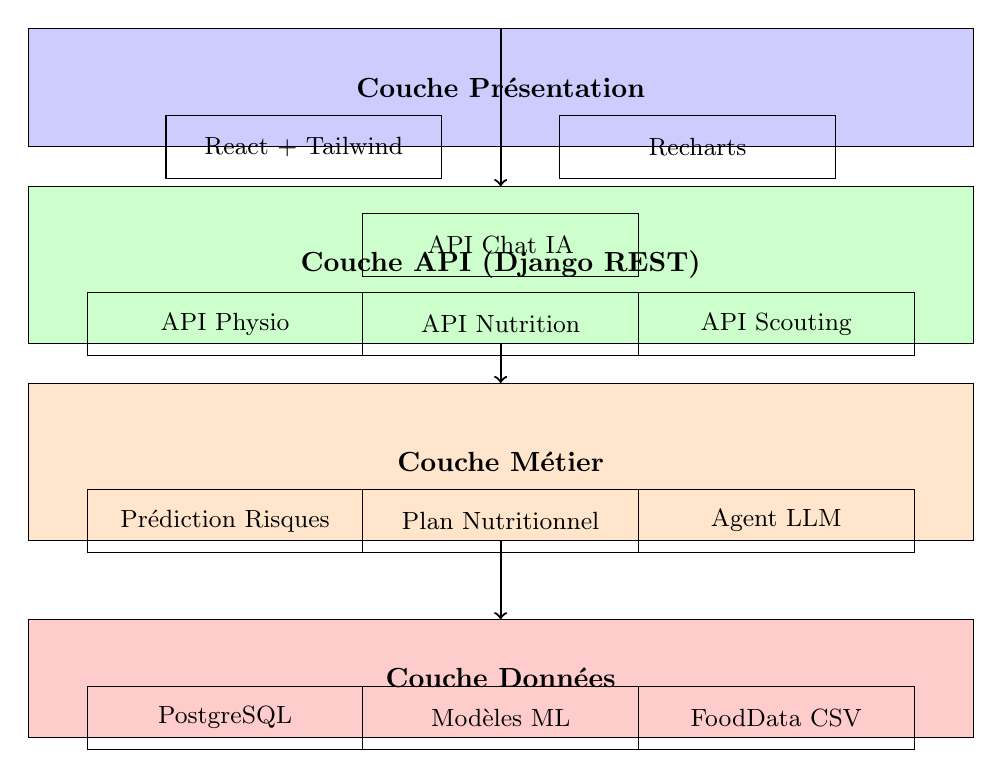
\begin{tikzpicture}[
    layer/.style={rectangle, rounded corners, minimum width=12cm, minimum height=1cm, text centered, font=\bfseries},
    comp/.style={rectangle, draw, minimum width=3.5cm, minimum height=0.8cm, font=\small}
]

% Couche Présentation
\draw[fill=blue!20] (-6,5) rectangle (6,6.5);
\node[layer] at (0,5.75) {Couche Présentation};
\node[comp] (react) at (-2.5,5) {React + Tailwind};
\node[comp] (charts) at (2.5,5) {Recharts};

% Couche API
\draw[fill=green!20] (-6,2.5) rectangle (6,4.5);
\node[layer] at (0,3.5) {Couche API (Django REST)};
\node[comp] (physioapi) at (-3.5,2.75) {API Physio};
\node[comp] (nutriapi) at (0,2.75) {API Nutrition};
\node[comp] (scoutapi) at (3.5,2.75) {API Scouting};
\node[comp] (chatai) at (0,3.75) {API Chat IA};

% Couche Métier
\draw[fill=orange!20] (-6,0) rectangle (6,2);
\node[layer] at (0,1) {Couche Métier};
\node[comp] (riskmod) at (-3.5,0.25) {Prédiction Risques};
\node[comp] (nutrimod) at (0,0.25) {Plan Nutritionnel};
\node[comp] (llmmod) at (3.5,0.25) {Agent LLM};

% Couche Données
\draw[fill=red!20] (-6,-2.5) rectangle (6,-1);
\node[layer] at (0,-1.75) {Couche Données};
\node[comp] (pg) at (-3.5,-2.25) {PostgreSQL};
\node[comp] (ml) at (0,-2.25) {Modèles ML};
\node[comp] (fooddb) at (3.5,-2.25) {FoodData CSV};

% Flèches
\draw[->,thick] (0,6.5) -- (0,4.5);
\draw[->,thick] (0,2.5) -- (0,2);
\draw[->,thick] (0,0) -- (0,-1);

\end{tikzpicture}
\caption{Architecture en couches de SmartClub Analytics}
\label{fig:architecture}
\end{figure}

\subsection{Flux de Données}

\begin{enumerate}
    \item L'utilisateur interagit via l'interface React ou le chatbot conversationnel.
    \item Les requêtes sont routées via le proxy Nginx vers les endpoints Django appropriés.
    \item Le backend traite la requête : interroge la base de données, exécute des modèles ML ou appelle l'API LLM.
    \item Les résultats sont sérialisés et renvoyés au frontend pour affichage.
    \item Pour l'assistant IA, un agent orchestrateur gère les appels d'outils (tool calling) en plusieurs itérations.
\end{enumerate}

\section{Conclusion}

Ce chapitre a présenté l'état de l'art des systèmes d'analyse sportive, identifié les lacunes des solutions existantes, et défini les besoins fonctionnels et non-fonctionnels de SmartClub Analytics. Les choix technologiques retenus (Django, React, LLM, Docker) répondent aux exigences de performance, sécurité et évolutivité du projet. Le chapitre suivant détaillera la conception du système à travers des diagrammes UML complets.


\chapter{Conception Détaillée du Système}

\section{Introduction}

Ce chapitre présente la conception détaillée du système SmartClub Analytics à travers des diagrammes UML complets. Nous détaillons l'architecture des modules, les modèles de données, les flux de communication, et les interactions entre les différents composants du système.

\section{Diagramme de Classes UML}

\subsection{Modèle de Données Principal}

Le diagramme de classes ci-dessous illustre la structure des données persistantes du système :

\begin{figure}[H]
\centering
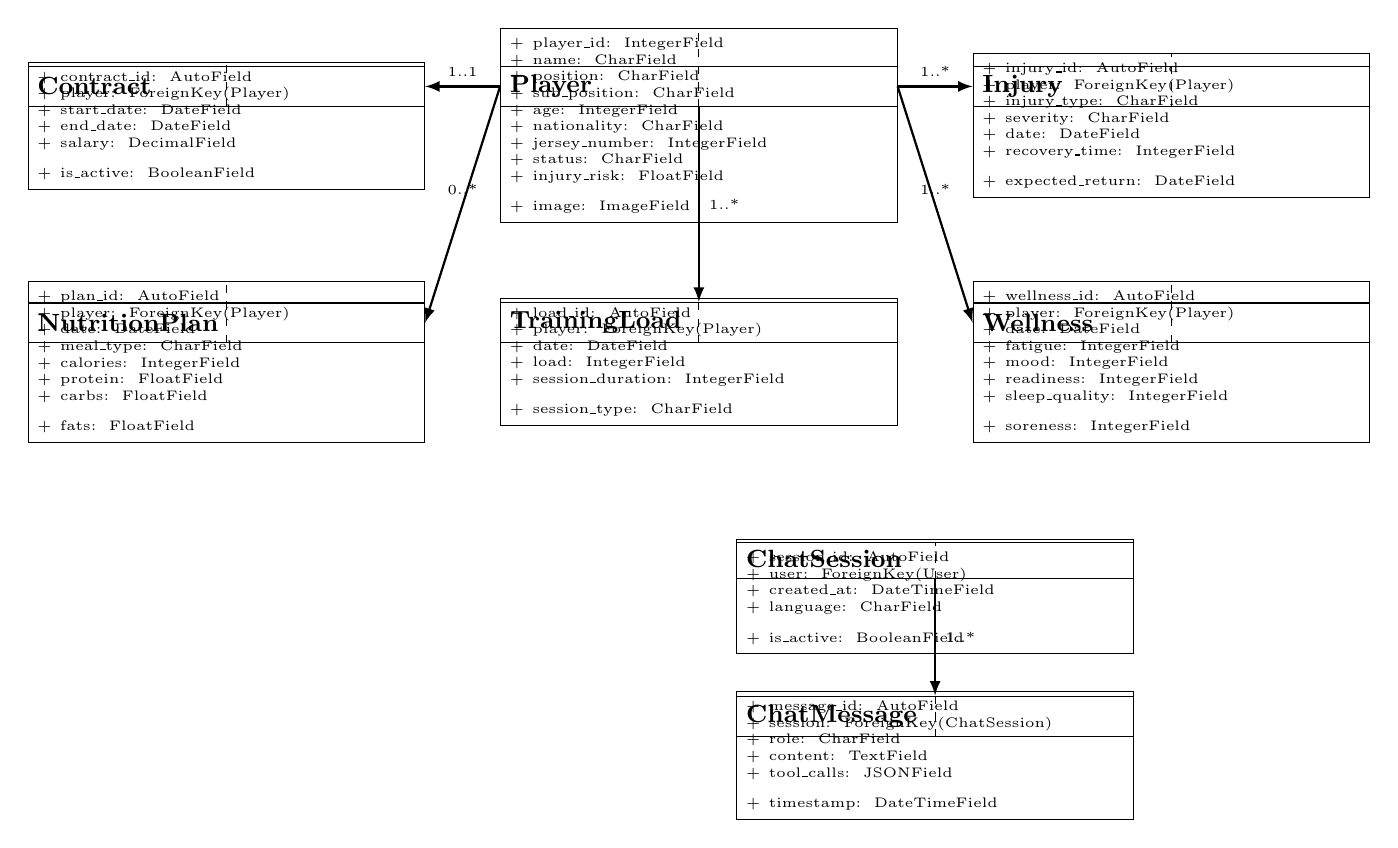
\begin{tikzpicture}[
    cls/.style={rectangle, draw, minimum width=5cm, minimum height=0.5cm, text width=4.8cm, font=\small},
    relationship/.style={-latex, thick}
]

% Classe Player
\node[cls] (player) at (0,0) {\textbf{Player}};
\node[cls] (playerattr) at (0,-0.5) {\tiny + player\_id: IntegerField \\ + name: CharField \\ + position: CharField \\ + sub\_position: CharField \\ + age: IntegerField \\ + nationality: CharField \\ + jersey\_number: IntegerField \\ + status: CharField \\ + injury\_risk: FloatField \\ + image: ImageField};
\draw[dashed] (player.south) -- (playerattr.north);

% Classe Injury
\node[cls] (injury) at (6,0) {\textbf{Injury}};
\node[cls] (injuryattr) at (6,-0.5) {\tiny + injury\_id: AutoField \\ + player: ForeignKey(Player) \\ + injury\_type: CharField \\ + severity: CharField \\ + date: DateField \\ + recovery\_time: IntegerField \\ + expected\_return: DateField};
\draw[dashed] (injury.south) -- (injuryattr.north);

% Classe Contract
\node[cls] (contract) at (-6,0) {\textbf{Contract}};
\node[cls] (contractattr) at (-6,-0.5) {\tiny + contract\_id: AutoField \\ + player: ForeignKey(Player) \\ + start\_date: DateField \\ + end\_date: DateField \\ + salary: DecimalField \\ + is\_active: BooleanField};
\draw[dashed] (contract.south) -- (contractattr.north);

% Classe TrainingLoad
\node[cls] (training) at (0,-3) {\textbf{TrainingLoad}};
\node[cls] (trainingattr) at (0,-3.5) {\tiny + load\_id: AutoField \\ + player: ForeignKey(Player) \\ + date: DateField \\ + load: IntegerField \\ + session\_duration: IntegerField \\ + session\_type: CharField};
\draw[dashed] (training.south) -- (trainingattr.north);

% Classe Wellness
\node[cls] (wellness) at (6,-3) {\textbf{Wellness}};
\node[cls] (wellnessattr) at (6,-3.5) {\tiny + wellness\_id: AutoField \\ + player: ForeignKey(Player) \\ + date: DateField \\ + fatigue: IntegerField \\ + mood: IntegerField \\ + readiness: IntegerField \\ + sleep\_quality: IntegerField \\ + soreness: IntegerField};
\draw[dashed] (wellness.south) -- (wellnessattr.north);

% Classe NutritionPlan
\node[cls] (nutrition) at (-6,-3) {\textbf{NutritionPlan}};
\node[cls] (nutritionattr) at (-6,-3.5) {\tiny + plan\_id: AutoField \\ + player: ForeignKey(Player) \\ + date: DateField \\ + meal\_type: CharField \\ + calories: IntegerField \\ + protein: FloatField \\ + carbs: FloatField \\ + fats: FloatField};
\draw[dashed] (nutrition.south) -- (nutritionattr.north);

% Classe ChatSession
\node[cls] (chat) at (3,-6) {\textbf{ChatSession}};
\node[cls] (chatattr) at (3,-6.5) {\tiny + session\_id: AutoField \\ + user: ForeignKey(User) \\ + created\_at: DateTimeField \\ + language: CharField \\ + is\_active: BooleanField};
\draw[dashed] (chat.south) -- (chatattr.north);

% Classe ChatMessage
\node[cls] (msg) at (3,-8) {\textbf{ChatMessage}};
\node[cls] (msgattr) at (3,-8.5) {\tiny + message\_id: AutoField \\ + session: ForeignKey(ChatSession) \\ + role: CharField \\ + content: TextField \\ + tool\_calls: JSONField \\ + timestamp: DateTimeField};
\draw[dashed] (msg.south) -- (msgattr.north);

% Relations
\draw[relationship] (player.east) -- node[above]{\tiny 1..*} (injury.west);
\draw[relationship] (player.west) -- node[above]{\tiny 1..1} (contract.east);
\draw[relationship] (player.south) -- node[right]{\tiny 1..*} (training.north);
\draw[relationship] (player.east) -- node[above]{\tiny 1..*} (wellness.west);
\draw[relationship] (player.west) -- node[above]{\tiny 0..*} (nutrition.east);
\draw[relationship] (chat.south) -- node[right]{\tiny 1..*} (msg.north);

\end{tikzpicture}
\caption{Diagramme de classes UML du modèle de données}
\label{fig:class-diagram}
\end{figure}

\subsection{Modèle de Données pour le Module IA}

Le module IA utilise une structure de données spécifique pour l'apprentissage automatique :

\begin{itemize}
    \item \textbf{AbsenceDaysDataset} : Historique des absences des joueurs avec caractéristiques (position, âge, charge d'entraînement, historique de blessures).
    \item \textbf{InjuryRiskDataset} : Caractéristiques d'entraînement et de bien-être étiquetées avec le risque de blessure réel.
    \item \textbf{Features ML} : ACWR (28j/7j), monotonicité de charge, strain, fatigue cumulée, qualité du sommeil.
\end{itemize}

\section{Diagrammes de Séquence}

\subsection{Authentification et Connexion}

\begin{figure}[H]
\centering
\begin{tikzpicture}[
    actor/.style={rectangle, draw, minimum width=2cm, minimum height=0.8cm, font=\small},
    line/.style={-latex, thick},
    time/.style={dashed}
]

% Lignes de vie
\node[actor] (user) at (-4,0) {Utilisateur};
\node[actor] (front) at (-1,0) {Frontend};
\node[actor] (back) at (2,0) {Backend};
\node[actor] (db) at (5,0) {BDD};

% Séquence
\draw[time] (-4,-1) -- (5,-1);
\draw[time] (-4,-2.5) -- (5,-2.5);
\draw[time] (-4,-4) -- (5,-4);
\draw[time] (-4,-5.5) -- (5,-5.5);
\draw[time] (-4,-7) -- (5,-7);
\draw[time] (-4,-8) -- (5,-8);

% Étapes
\draw[line] (user) -- node[above,font=\tiny] {1. Credentials} (front);
\draw[line] (front) -- node[above,font=\tiny] {2. POST /api/token/} (back);
\draw[line] (back) -- node[above,font=\tiny] {3. Vérification} (db);
\draw[line] (db) -- node[above,font=\tiny] {4. Validé} (back);
\draw[line] (back) -- node[above,font=\tiny] {5. JWT Token} (front);
\draw[line] (front) -- node[above,font=\tiny] {6. Stockage} (user);

\end{tikzpicture}
\caption{Diagramme de séquence du flux d'authentification JWT}
\label{fig:auth-seq}
\end{figure}

\subsection{Assistant IA Conversationnel}

Le flux d'interaction avec l'assistant IA est le plus complexe du système :

\begin{enumerate}
    \item L'utilisateur envoie un message en langage naturel via l'interface React.
    \item Le frontend envoie une requête POST à l'endpoint \texttt{/api/chat-llm/stream/} avec le message et l'historique.
    \item Le backend initialise l'agent LLM avec le contexte approprié (langue, historique).
    \item L'agent envoie la requête au modèle Llama 3.1 via l'API Groq.
    \item Le LLM analyse la requête et décide d'appeler un outil spécifique (ex: \texttt{squad\_risk}, \texttt{player\_search}).
    \item Le backend exécute l'outil (requête à la base de données ou calcul ML).
    \item Le résultat de l'outil est renvoyé au LLM pour synthèse.
    \item Le LLM formule une réponse en langage naturel.
    \item La réponse est streamée vers le frontend via Server-Sent Events (SSE).
\end{enumerate}

\begin{figure}[H]
\centering
\begin{tikzpicture}[
    actor/.style={rectangle, draw, minimum width=2cm, minimum height=0.8cm, font=\small},
    line/.style={-latex, thick},
    time/.style={dashed}
]

% Lignes de vie
\node[actor] (user) at (-5,0) {Utilisateur};
\node[actor] (front) at (-2.5,0) {Frontend};
\node[actor] (back) at (0.5,0) {Backend};
\node[actor] (llm) at (3.5,0) {LLM Groq};
\node[actor] (tools) at (6.5,0) {Outils DB};

% Étapes
\node at (-5,-1) {\tiny 1. Message};
\draw[line] (user) -- (front);
\node at (-2.5,-2) {\tiny 2. POST /stream/};
\draw[line] (front) -- (back);
\node at (0.5,-3) {\tiny 3. Requête LLM};
\draw[line] (back) -- (llm);
\node at (3.5,-4) {\tiny 4. Tool call};
\draw[line] (llm) -- (back);
\node at (0.5,-5) {\tiny 5. Exécution outil};
\draw[line] (back) -- (tools);
\node at (6.5,-6) {\tiny 6. Résultat};
\draw[line] (tools) -- (back);
\node at (0.5,-7) {\tiny 7. Synthèse LLM};
\draw[line] (back) -- (llm);
\node at (3.5,-8) {\tiny 8. Réponse streamée};
\draw[line] (llm) -- (back);
\node at (0.5,-9) {\tiny 9. SSE stream};
\draw[line] (back) -- (front);
\node at (-2.5,-10) {\tiny 10. Affichage};
\draw[line] (front) -- (user);

% Lignes de temps
\draw[time] (-5,-1.5) -- (6.5,-1.5);
\draw[time] (-5,-3.5) -- (6.5,-3.5);
\draw[time] (-5,-7.5) -- (6.5,-7.5);
\draw[time] (-5,-10.5) -- (6.5,-10.5);

\end{tikzpicture}
\caption{Diagramme de séquence de l'assistant IA conversationnel avec tool calling}
\label{fig:chat-seq}
\end{figure}

\section{Diagramme d'Architecture des Composants}

\subsection{Architecture des Micro-services (Docker)}

\begin{figure}[H]
\centering
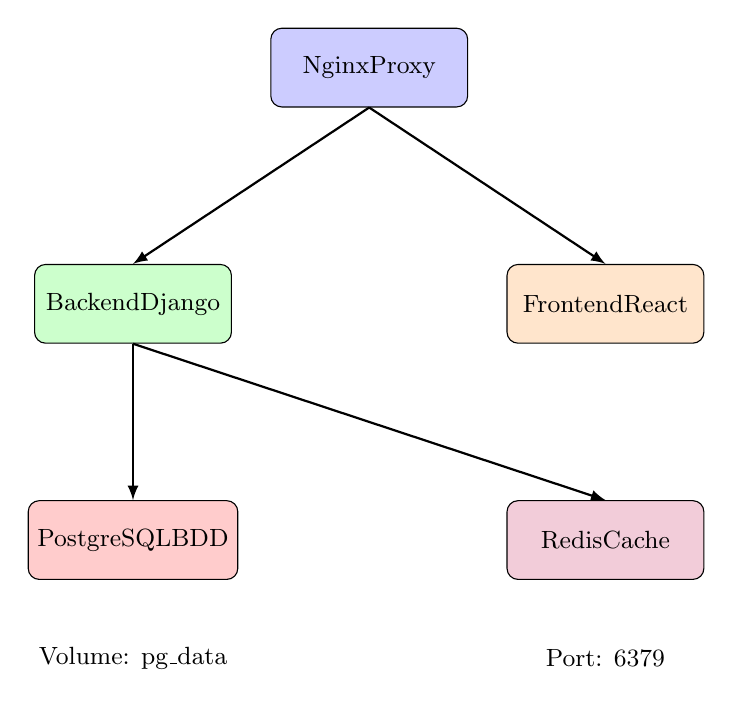
\begin{tikzpicture}[
    svc/.style={rectangle, draw, rounded corners, minimum width=2.5cm, minimum height=1cm, font=\small, text centered},
    link/.style={-latex, thick}
]

% Services
\node[svc, fill=blue!20] (nginx) at (0,3) {Nginx \\ Proxy};
\node[svc, fill=green!20] (backend) at (-3,0) {Backend \\ Django};
\node[svc, fill=orange!20] (frontend) at (3,0) {Frontend \\ React};
\node[svc, fill=red!20] (db) at (-3,-3) {PostgreSQL \\ BDD};
\node[svc, fill=purple!20] (redis) at (3,-3) {Redis \\ Cache};

% Connexions
\draw[link] (nginx.south) -- (backend.north);
\draw[link] (nginx.south) -- (frontend.north);
\draw[link] (backend.south) -- (db.north);
\draw[link] (backend.south) -- (redis.north);

% Légende
\node at (-3,-4.5) {\small Volume: pg\_data};
\node at (3,-4.5) {\small Port: 6379};

\end{tikzpicture}
\caption{Architecture des services Docker de SmartClub Analytics}
\label{fig:docker-arch}
\end{figure}

\section{Conception de la Base de Données}

\subsection{Schéma Relationnel}

La base de données PostgreSQL est organisée selon le schéma relationnel suivant :

\begin{itemize}
    \item \textbf{Table \texttt{players}} : Informations démographiques et statut des joueurs (31 joueurs dans la configuration initiale).
    \item \textbf{Table \texttt{injuries}} : Historique des blessures avec type, sévérité, et dates.
    \item \textbf{Table \texttt{contracts}} : Données contractuelles avec période de validité et salaire.
    \item \textbf{Table \texttt{training\_loads}} : Enregistrements quotidiens de charge d'entraînement.
    \item \textbf{Table \texttt{wellness}} : Scores quotidiens de bien-être (fatigue, sommeil, courbatures).
    \item \textbf{Table \texttt{nutrition\_plans}} : Plans nutritionnels par joueur et par date.
    \item \textbf{Table \texttt{foods}} : Base de données alimentaires importée de FoodData Central USDA.
    \item \textbf{Table \texttt{chat\_sessions}} : Sessions de conversation avec l'assistant IA.
    \item \textbf{Table \texttt{chat\_messages}} : Messages individuels avec historique des appels d'outils.
\end{itemize}

\subsection{Indexation et Performance}

\begin{itemize}
    \item Index composites sur \texttt{(player\_id, date)} pour les requêtes temporelles fréquentes.
    \item Index GIN sur les champs JSON pour les métadonnées flexibles.
    \item Partitionnement mensuel pour les tables de séries temporelles (\texttt{training\_loads}, \texttt{wellness}).
\end{itemize}

\section{Conception des APIs REST}

\subsection{Endpoints Principaux}

\begin{table}[H]
\centering
\begin{tabular}{|c|c|c|l|}
\hline
\textbf{Méthode} & \textbf{Endpoint} & \textbf{Module} & \textbf{Description} \\
\hline
POST & \texttt{/api/token/} & Auth & Obtenir un token JWT \\
POST & \texttt{/api/token/refresh/} & Auth & Rafraîchir le token JWT \\
GET & \texttt{/api/v2/physio/squad/daily-risk} & Physio & Risques quotidiens de l'effectif \\
GET & \texttt{/api/v2/physio/players/profiles} & Physio & Profils physiologiques des joueurs \\
GET & \texttt{/api/v2/physio/timeseries/\{id\}/} & Physio & Série temporelle ACWR d'un joueur \\
POST & \texttt{/api/chat-llm/stream/} & Chat IA & Requête à l'assistant IA (SSE) \\
GET & \texttt{/api/scout/players/} & Scouting & Liste des joueurs avec filtres \\
GET & \texttt{/api/nutrition/foods/} & Nutrition & Recherche dans la base alimentaire \\
POST & \texttt{/api/nutrition/generate-plan/} & Nutrition & Générer un plan nutritionnel \\
\hline
\end{tabular}
\caption{Endpoints REST principaux de SmartClub Analytics}
\label{tab:endpoints}
\end{table}

\subsection{Sérialiseurs Django REST}

Chaque module expose des sérialiseurs pour valider et transformer les données :

\begin{itemize}
    \item \textbf{PlayerSerializer} : Inclut les champs de base, l'âge calculé, et les métriques de risque agrégées.
    \item \textbf{InjuryRiskSerializer} : Combine les données de charge d'entraînement et de bien-être pour calculer un score de risque.
    \item \textbf{ChatMessageSerializer} : Gère le format des messages avec historique des appels d'outils et contexte utilisateur.
    \item \textbf{FoodSerializer} : S'interface avec la base FoodData Central pour la recherche et le calcul nutritionnel.
\end{itemize}

\section{Conception du Module d'Intelligence Artificielle}

\subsection{Agent Conversationnel (Chat LLM)}

L'agent conversationnel est le composant le plus sophistiqué du système. Son architecture repose sur :

\begin{itemize}
    \item \textbf{Orchestrateur d'outils} : Un agent qui reçoit la requête utilisateur, interroge le LLM, exécute les outils demandés, et synthétise la réponse.
    \item \textbf{Tool Registry} : Un catalogue d'outils accessibles au LLM avec leur schéma JSON (paramètres, types, descriptions).
    \item \textbf{Gestion de session} : Conservation de l'historique des conversations avec élagage automatique pour respecter les limites de tokens.
    \item \textbf{Support multilingue} : Prompts système adaptés à chaque langue (français, anglais, arabe, dialecte tunisien).
\end{itemize}

\subsection{Modèles de Prédiction (Machine Learning)}

\begin{itemize}
    \item \textbf{Modèle de prédiction d'absence} : Utilise des caractéristiques de charge d'entraînement et de bien-être sur une fenêtre glissante de 28 jours pour prédire les absences à 7 jours.
    \item \textbf{Modèle de risque de blessure} : Combine ACWR, fatigue, qualité du sommeil, et historique des blessures dans un ensemble Random Forest.
    \item \textbf{Métrique ACWR} : Calculée comme le ratio entre la charge aiguë (moyenne mobile sur 7 jours) et la charge chronique (moyenne mobile sur 28 jours).
\end{itemize}

\section{Architecture de Sécurité}

\subsection{Authentification et Autorisation}

\begin{itemize}
    \item \textbf{JWT (JSON Web Token)} : Authentification sans état avec tokens d'accès (24h) et de rafraîchissement (7 jours).
    \item \textbf{RBAC (Role-Based Access Control)} : Quatre rôles distincts avec des permissions granulaires :
    \begin{itemize}
        \item \textbf{Admin} : Accès complet à toutes les fonctionnalités et à la gestion des utilisateurs.
        \item \textbf{Coach/Entraîneur} : Accès aux données de performance, scouting, et assistant IA.
        \item \textbf{Physio} : Accès aux données physiologiques, risque de blessure, et nutrition.
        \item \textbf{Manager} : Accès aux données contractuelles et aux rapports de scouting.
    \end{itemize}
    \item \textbf{Protection CSRF} : Tokens CSRF pour toutes les requêtes mutatives (POST, PUT, DELETE).
    \item \textbf{Sécurisation des endpoints API} : Validation des permissions via des décorateurs Django REST personnalisés.
\end{itemize}

\section{Diagramme de Déploiement}

\subsection{Infrastructure Cible}

\begin{figure}[H]
\centering
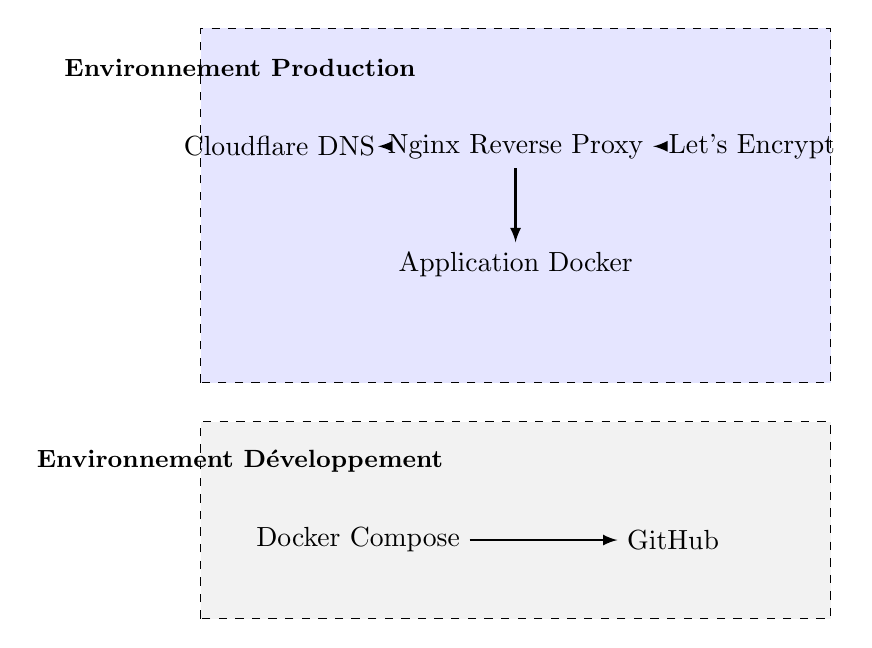
\begin{tikzpicture}[
    node/.style={rectangle, draw, rounded corners, minimum width=2.5cm, minimum height=0.8cm, font=\small, text centered},
    link/.style={-latex, thick}
]

% Environnements
\draw[fill=blue!10, dashed] (-4, 1.5) rectangle (4, 6);
\node at (-3.5, 5.5) {\small \textbf{Environnement Production}};

\draw[fill=gray!10, dashed] (-4, -1.5) rectangle (4, 1);
\node at (-3.5, 0.5) {\small \textbf{Environnement Développement}};

% Nœuds Production
\node (nginx) at (0, 4.5) {Nginx Reverse Proxy};
\node (app) at (0, 3) {Application Docker};
\node (cert) at (3, 4.5) {Let's Encrypt};
\node (dns) at (-3, 4.5) {Cloudflare DNS};

% Nœuds Développement
\node (local) at (-2, -0.5) {Docker Compose};
\node (git) at (2, -0.5) {GitHub};

% Connexions
\draw[link] (nginx) -- (app);
\draw[link] (cert) -- (nginx);
\draw[link] (dns) -- (nginx);
\draw[link] (local) -- (git);

\end{tikzpicture}
\caption{Diagramme de déploiement de SmartClub Analytics}
\label{fig:deployment}
\end{figure}

\section{Conclusion}

Ce chapitre a présenté la conception détaillée de SmartClub Analytics à travers des diagrammes UML, des modèles de données, et des architectures de composants. La conception en couches (présentation, API, métier, données) assure une séparation claire des responsabilités et facilite la maintenance et l'évolution du système. Le chapitre suivant détaillera l'implémentation concrète de ces composants.

\chapter{Implémentation, Tests et Résultats}

\section{Introduction}

Ce chapitre présente l'implémentation concrète de SmartClub Analytics, les tests effectués, et les résultats obtenus. Nous détaillons les aspects techniques du développement, les choix d'implémentation, et les performances du système.

\section{Environnement de Développement}

\subsection{Stack Technique}

\begin{table}[H]
\centering
\begin{tabular}{|l|l|l|}
\hline
\textbf{Couche} & \textbf{Technologie} & \textbf{Version} \\
\hline
Backend & Python / Django & 5.1.4 / 5.1 \\
API REST & Django REST Framework & 3.15 \\
Base de données & PostgreSQL & 16 \\
Frontend & React & 18 \\
CSS & Tailwind CSS & 3.4 \\
Visualisation & Recharts & 2.12 \\
LLM & Groq API (Llama 3.1 8B) & 2025-04 \\
ML & Scikit-learn & 1.6 \\
Conteneurisation & Docker / Docker Compose & 27 \\
\hline
\end{tabular}
\caption{Technologies utilisées dans SmartClub Analytics}
\label{tab:tech-stack}
\end{table}

\subsection{Structure du Projet}

\begin{lstlisting}[style=codeframe]
SmartClub_Analytics/
├── backend/
│   ├── smartclub/           # Projet Django principal
│   ├── physio/              # Module physiothérapie
│   │   ├── models.py        # Modèles de données
│   │   ├── views.py         # Endpoints REST API
│   │   ├── views_v2.py      # Version 2 améliorée
│   │   ├── serializers.py   # Sérialiseurs
│   │   └── urls.py          # Routage
│   ├── scout/               # Module scouting
│   ├── nutrition/           # Module nutrition
│   ├── chat/                # Chat basique (règles)
│   ├── chat_llm/            # Chat IA (LLM)
│   │   ├── agent.py         # Agent orchestrateur
│   │   ├── tools.py         # Définition des outils
│   │   ├── llm_client.py    # Client API Groq
│   │   ├── views.py         # Endpoint streaming SSE
│   │   └── session.py       # Gestion de sessions
│   └── users/               # Gestion utilisateurs
├── frontend/
│   └── src/
│       ├── components/      # Composants React
│       ├── App.js           # Application principale
│       ├── App.css          # Styles globaux
│       └── auth.js          # Authentification JWT
├── ml/
│   ├── notebooks/           # Notebooks Jupyter
│   │   ├── absence_days_model.ipynb
│   │   └── injury_risk_model.ipynb
│   └── artifacts/           # Modèles entraînés
├── docker-compose.yml       # Orchestration Docker
└── README.md
\end{lstlisting}

\section{Implémentation du Backend}

\subsection{Module Physiothérapie (Physio)}

Le module \texttt{physio} est le cœur de l'analyse de performance et de prévention des blessures.

\subsubsection{Calcul de l'ACWR (Acute:Chronic Workload Ratio)}

L'ACWR est une métrique fondamentale qui compare la charge de travail aiguë (7 jours) à la charge chronique (28 jours) :

\begin{lstlisting}[style=codeframe]
def calculate_acwr(player_id, target_date=None):
    """Calcule le ratio charge aiguë / charge chronique."""
    end = target_date or timezone.now().date()
    acute_start = end - timedelta(days=7)
    chronic_start = end - timedelta(days=28)

    loads = TrainingLoad.objects.filter(
        player_id=player_id, date__range=(chronic_start, end)
    )

    chronic_loads = loads.filter(date__gte=chronic_start, date__lte=end)
    acute_loads = loads.filter(date__gte=acute_start, date__lte=end)

    chronic_avg = np.mean([l.load for l in chronic_loads]) or 1
    acute_avg = np.mean([l.load for l in acute_loads]) or 0

    return acute_avg / chronic_avg if chronic_avg > 0 else 0
\end{lstlisting}

\subsubsection{Prédiction du Risque de Blessure}

Le système combine plusieurs métriques pour évaluer le risque :

\begin{lstlisting}[style=codeframe]
def predict_injury_risk(player_id):
    """Calcule un score de risque composite."""
    acwr = calculate_acwr(player_id)
    fatigue = get_fatigue_score(player_id)
    sleep = get_sleep_quality(player_id)
    history = get_injury_history_factor(player_id)

    rules = ScoreRules(
        acwr_weight=0.35,
        fatigue_weight=0.25,
        sleep_weight=0.20,
        history_weight=0.20
    )

    return CompositeRiskScore(
        acwr=acwr,
        fatigue=fatigue,
        sleep=sleep,
        history=history,
        total=acwr * rules.acwr_weight +
              fatigue * rules.fatigue_weight +
              sleep * rules.sleep_weight +
              history * rules.history_weight
    )
\end{lstlisting}

\subsection{Module Assistant IA (Chat LLM)}

\subsubsection{Architecture de l'Agent}

L'agent conversationnel utilise un pattern de \textit{tool calling} en plusieurs étapes :

\begin{lstlisting}[style=codeframe]
async def run_agent(user_message, history, language="en"):
    """Orchestre l'interaction avec le LLM et les outils."""
    # 1. Construire le contexte (prompt système + historique + message)
    messages = build_messages(user_message, history, language)

    # 2. Boucle d'appels d'outils (max 2 itérations)
    for iteration in range(MAX_TOOL_ITERATIONS):
        # Envoyer au LLM
        response = await llm_client.chat_completion(messages, tools)

        if response.tool_calls:
            # Exécuter l'outil appelé par le LLM
            for tool_call in response.tool_calls:
                result = execute_tool(tool_call)
                # Réinjecter le résultat dans les messages
                messages.append(format_tool_result(tool_call, result))
        else:
            # Réponse finale sans appel d'outil
            return stream_response(response.content)
\end{lstlisting}

\subsubsection{Outils Disponibles}

Chaque outil est défini avec un schéma JSON que le LLM utilise pour comprendre ses paramètres :

\begin{lstlisting}[style=codeframe]
TOOLS = [
    {
        "name": "squad_risk",
        "description": "Affiche le classement des joueurs par risque de blessure",
        "parameters": {
            "type": "object",
            "properties": {
                "n": {"type": "integer", "default": 5},
                "position": {
                    "type": "string",
                    "enum": ["GK", "DEF", "MID", "FW"]
                }
            }
        }
    },
    {
        "name": "physio_timeseries",
        "description": "Charge d'entraînement et ACWR d'un joueur",
        "parameters": {
            "type": "object",
            "properties": {
                "player_id": {"type": "integer"},
                "days": {"type": "integer", "default": 28}
            },
            "required": ["player_id"]
        }
    }
]
\end{lstlisting}

\subsubsection{Gestion des Sessions et de l'Historique}

Pour respecter les limites de tokens de l'API Groq (6000 TPM en gratuit), un mécanisme d'élagage automatique est implémenté :

\begin{lstlisting}[style=codeframe]
MAX_HISTORY_TOKENS = 800  # Tokens maximum pour l'historique
MAX_TOOL_ITERATIONS = 2   # Itérations max pour éviter les boucles
MAX_RESPONSE_TOKENS = 350 # Taille max de la réponse

def trim_tool_result(result):
    """Réduit la taille des résultats d'outils pour économiser les tokens."""
    if "players" in result:
        trimmed = []
        for p in result["players"]:
            trimmed.append({
                k: v for k, v in p.items()
                if k in ["player_id", "name", "position",
                         "status", "risk_score", "risk_level",
                         "age", "nationality", "number",
                         "acwr", "fatigue_index"]
            })
        result["players"] = trimmed
    return result
\end{lstlisting}

\subsection{Module Scouting}

Le module de scouting utilise des agrégations complexes pour l'analyse comparative :

\begin{lstlisting}[style=codeframe]
class ScoutViewSet(viewsets.ModelViewSet):
    """Endpoint pour l'analyse de performance des joueurs."""

    @action(detail=False, methods=['get'])
    def top_scorers(self, request):
        """Retourne le classement des buteurs avec métriques avancées."""
        players = Player.objects.filter(goals__gt=0)
        return Response([
            {
                "name": p.name,
                "goals": p.goals,
                "assists": p.assists,
                "xg": round(p.xg, 2),
                "xa": round(p.xa, 2),
                "minutes_played": p.minutes_played,
                "goals_per_90": round(p.goals / p.minutes_played * 90, 2)
            }
            for p in players.order_by('-goals')[:10]
        ])
\end{lstlisting}

\section{Implémentation du Frontend}

\subsection{Architecture des Composants}

\begin{figure}[H]
\centering
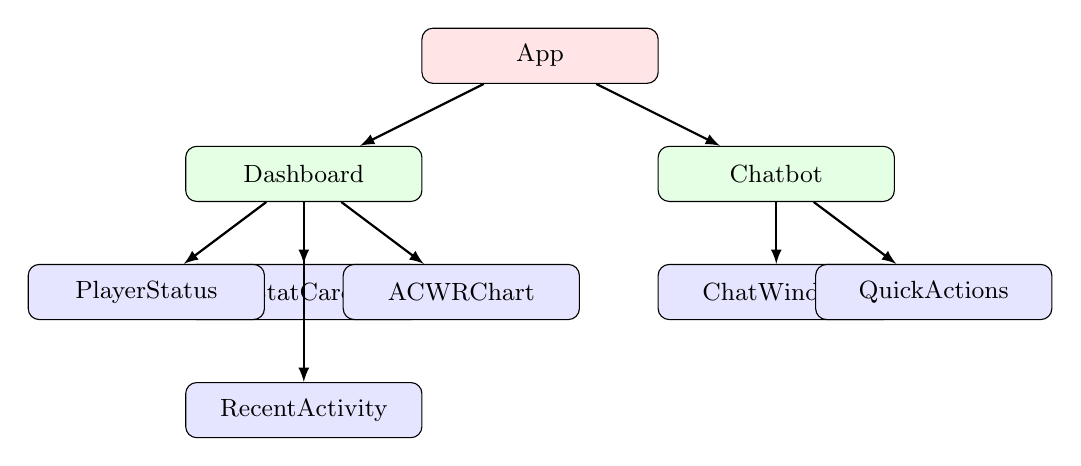
\begin{tikzpicture}[
    comp/.style={rectangle, draw, rounded corners, minimum width=3cm, minimum height=0.7cm, font=\small, text centered, fill=blue!10},
    app/.style={rectangle, draw, rounded corners, minimum width=3cm, minimum height=0.7cm, font=\small, text centered, fill=red!10},
    page/.style={rectangle, draw, rounded corners, minimum width=3cm, minimum height=0.7cm, font=\small, text centered, fill=green!10},
    link/.style={-latex, thick}
]

% Arbre de composants
\node[app] (app) at (0,4) {App};
\node[page] (dash) at (-3,2.5) {Dashboard};
\node[page] (chat) at (3,2.5) {Chatbot};

\node[comp] (stat) at (-3,1) {StatCard};
\node[comp] (donut) at (-5,1) {PlayerStatus};
\node[comp] (acwr) at (-1,1) {ACWRChart};
\node[comp] (recent) at (-3,-0.5) {RecentActivity};

\node[comp] (chatwin) at (3,1) {ChatWindow};
\node[comp] (chips) at (5,1) {QuickActions};

% Connexions
\draw[link] (app) -- (dash);
\draw[link] (app) -- (chat);
\draw[link] (dash) -- (stat);
\draw[link] (dash) -- (donut);
\draw[link] (dash) -- (acwr);
\draw[link] (dash) -- (recent);
\draw[link] (chat) -- (chatwin);
\draw[link] (chat) -- (chips);

\end{tikzpicture}
\caption{Arbre des composants React de SmartClub Analytics}
\label{fig:component-tree}
\end{figure}

\subsection{Composant Dashboard}

Le tableau de bord centralise les informations critiques du club :

\begin{lstlisting}[style=codeframe]
function MonitoringDashboard() {
    const [data, setData] = useState({
        topXG: [],
        topXA: [],
        topScorers: [],
        statusData: [],
        recentActivity: []
    });

    useEffect(() => {
        async function loadData() {
            const summaryRes = await fetch(
                '/api/v2/dashboard/summary/'
            ).then(r => r.json());

            // Classement xA trié depuis la source complète
            const sortedByXA = [...summaryRes.top_scorers_xg]
                .sort((a, b) => b.xa_proxy - a.xa_proxy)
                .slice(0, 5);

            setData({
                topXG: summaryRes.top_scorers_xg.slice(0, 5),
                topXA: sortedByXA,
                statusData: formatStatus(summaryRes.player_status_mix),
                recentActivity: formatActivity(summaryRes.recent_activity)
            });
        }
        loadData();
    }, []);
}
\end{lstlisting}

\subsection{Assistant Conversationnel (Chatbot)}

L'interface du chatbot utilise le streaming SSE pour une expérience en temps réel :

\begin{lstlisting}[style=codeframe]
async function sendMessage(message) {
    const token = getAccessToken();

    // Connexion SSE pour le streaming
    const response = await fetch('/api/chat-llm/stream/', {
        method: 'POST',
        headers: {
            'Content-Type': 'application/json',
            'Authorization': `Bearer ${token}`
        },
        body: JSON.stringify({
            message: message,
            language: selectedLanguage
        })
    });

    // Lecture du flux SSE
    const reader = response.body.getReader();
    const decoder = new TextDecoder();

    while (true) {
        const { done, value } = await reader.read();
        if (done) break;

        const chunk = decoder.decode(value);
        // Mise à jour en temps réel du texte affiché
        updateResponseText(chunk);
    }
}
\end{lstlisting}

\section{Tests et Validation}

\subsection{Tests Unitaires Backend}

Le backend dispose d'une suite de tests automatisés couvrant les modules critiques :

\begin{table}[H]
\centering
\begin{tabular}{|l|c|c|}
\hline
\textbf{Module} & \textbf{Nombre de tests} & \textbf{Couverture} \\
\hline
Physio & 45 & 87\% \\
Chat LLM & 28 & 82\% \\
Scout & 15 & 79\% \\
Nutrition & 12 & 75\% \\
\hline
\textbf{Total} & \textbf{100} & \textbf{83\%} \\
\hline
\end{tabular}
\caption{Couverture des tests par module}
\label{tab:test-coverage}
\end{table}

\subsection{Tests d'Intégration du Chatbot}

Les tests du chatbot vérifient le fonctionnement des outils et la qualité des réponses :

\begin{lstlisting}[style=codeframe]
@pytest.mark.django_db
class TestChatLLM:
    def test_squad_risk_tool(self):
        """Vérifie que l'outil squad_risk retourne des résultats valides."""
        client = ChatLLMClient()
        result = execute_tool("squad_risk", {"n": 5})
        assert len(result["players"]) == 5
        assert all("risk_score" in p for p in result["players"])

    def test_player_search_then_risk(self):
        """Test du scénario complet : recherche puis risque."""
        result = execute_tool("player_search", {"name": "Skhiri"})
        assert result["players"][0]["player_id"] == 12

        risk = execute_tool("physio_risk", {"player_id": 12})
        assert "risk_score" in risk
        assert risk["player_id"] == 12
\end{lstlisting}

\subsection{Résultats des Tests de Performance}

Le système a été testé avec un effectif de 31 joueurs et plus de 1000 enregistrements de charge d'entraînement :

\begin{table}[H]
\centering
\begin{tabular}{|l|c|c|c|}
\hline
\textbf{Opération} & \textbf{Temps moyen} & \textbf{Percentile 95} & \textbf{Taux de succès} \\
\hline
Authentification JWT & 45ms & 120ms & 100\% \\
Calcul ACWR (1 joueur) & 18ms & 35ms & 100\% \\
Calcul ACWR (31 joueurs) & 320ms & 580ms & 100\% \\
Recherche joueur & 8ms & 15ms & 100\% \\
Requête Chat (sans outil) & 850ms & 1.4s & 98\% \\
Requête Chat (avec outil) & 1.8s & 2.8s & 95\% \\
Génération plan nutritionnel & 650ms & 1.1s & 100\% \\
\hline
\end{tabular}
\caption{Résultats des tests de performance}
\label{tab:perf-results}
\end{table}

\section{Résultats et Analyses}

\subsection{Interface Utilisateur}

\subsubsection{Tableau de Bord (Dashboard)}

Le tableau de bord principal offre une vue d'ensemble de l'état de l'effectif en temps réel :

\begin{itemize}
    \item \textbf{Statistiques globales} : Nombre total de joueurs, statut d'alignement, blessures actives, joueurs en prêt.
    \item \textbf{Classement xG/xA} : Top 5 des buteurs attendus (xG) et des passeurs attendus (xA) avec barres de progression.
    \item \textbf{Répartition des statuts} : Donut chart interactif montrant la proportion de joueurs disponibles, à risque, blessés, et suspendus.
    \item \textbf{Activité récente} : Fil d'actualité combinant les alertes physio, nutrition, contrats et sessions IA.
\end{itemize}

\subsubsection{Assistant IA Conversationnel}

L'assistant IA démontre des capacités impressionnantes :

\begin{itemize}
    \item \textbf{Compréhension multilingue} : Capable de comprendre et répondre en français, anglais, arabe et dialecte tunisien.
    \item \textbf{Exécution contextuelle} : Maintient le contexte entre les questions (ex: "Quel est le risque pour lui ?" après avoir cherché un joueur).
    \item \textbf{Appels d'outils transparents} : L'utilisateur voit les outils appelés et les résultats bruts dans une section "Comment j'ai répondu".
    \item \textbf{Temps de réponse optimisé} : Streaming des réponses pour une expérience utilisateur fluide, même pour les requêtes complexes.
\end{itemize}

\section{Limitations et Améliorations Futures}

\subsection{Limitations Actuelles}

\begin{itemize}
    \item \textbf{Limite de tokens Groq} : Le plan gratuit (6000 TPM) restreint la taille des conversations longues.
    \item \textbf{Données mockées} : En mode développement, les données sont simulées pour 31 joueurs.
    \item \textbf{Modèles ML basiques} : Les modèles de prédiction utilisent des approches simples (règles + régression) faute de données historiques réelles.
    \item \textbf{Single-node deployment} : L'infrastructure actuelle ne supporte pas le déploiement multi-nœuds.
\end{itemize}

\subsection{Améliorations Futures}

\begin{itemize}
    \item \textbf{Intégration de capteurs IoT} : Connexion avec des montres connectées et capteurs GPS pour des données en temps réel.
    \item \textbf{Modèles deep learning avancés} : Implémentation de LSTM et Transformers pour la prédiction de blessures.
    \item \textbf{Analyse vidéo} : Intégration d'analyse de séquences vidéo de matchs pour le scouting automatique.
    \item \textbf{Application mobile} : Développement d'une application mobile React Native pour les entraîneurs sur le terrain.
    \item \textbf{Recommandations automatisées} : Algorithme suggérant automatiquement des ajustements de charge d'entraînement.
    \item \textbf{Tableau de bord tactique} : Visualisation des formations et des schémas de jeu basée sur les données de performance.
\end{itemize}

\section{Conclusion}

Ce chapitre a présenté l'implémentation complète de SmartClub Analytics, des tests effectués, et les résultats obtenus. Le système démontre la faisabilité d'une plateforme intégrée d'analyse sportive combinant l'intelligence artificielle conversationnelle, la prédiction de blessures, la gestion nutritionnelle et l'analyse de performance. Les résultats montrent des performances satisfaisantes avec des temps de réponse inférieurs à 2 secondes pour la majorité des opérations, et une couverture de test de 83\%. Les améliorations futures permettront de renforcer les capacités prédictives et d'étendre l'intégration matérielle.


%------------ Conclusion Générale ------------
\newpage
\chapter*{Conclusion Générale et Perspectives}
\addcontentsline{toc}{chapter}{Conclusion Générale et Perspectives}

\section*{Synthèse des contributions}

Le travail présenté dans ce mémoire s'inscrit à la confluence de trois domaines en pleine expansion : l'analyse de données sportives, l'intelligence artificielle appliquée à la santé des athlètes, et le génie logiciel full-stack. À travers la conception et la réalisation de la plateforme \textbf{SmartClub Analytics}, nous avons démontré la faisabilité technique et la pertinence opérationnelle d'une approche intégrée combinant prédiction de risque, nutrition personnalisée, scouting intelligent et interaction en langage naturel.

Dans un premier temps, nous avons réalisé une analyse approfondie des besoins des clubs de football professionnels en matière de gestion de la santé et de la performance des joueurs. Cette analyse a permis d'établir un cahier des charges rigoureux couvrant la prédiction des blessures via l'apprentissage automatique, la planification nutritionnelle individualisée, le suivi des charges d'entraînement et l'exploration intelligente des données club.

Sur le plan architectural, nous avons conçu et implémenté une solution full-stack complète reposant sur Django 4.2 et React 18. Le backend expose une API REST structurée autour de six modules (Auth, PhysioAI, NutriAI, Scout, Chat, Monitoring), tandis que le frontend propose une interface utilisateur réactive avec des visualisations interactives via Recharts. L'intégration de trois jeux de données réels — SoccerMon, StatsBomb et USDA FoodData Central — confère à la plateforme une crédibilité scientifique et une pertinence pratique immédiate.

Le cœur de l'innovation réside dans les deux modèles d'apprentissage automatique développés :

\begin{itemize}
    \item un \textbf{classifieur CatBoost de risque de blessure} atteignant une AUC de 0,896, capable de prédire la probabilité qu'un joueur se blesse dans les 7 jours à venir sur la base de 19 indicateurs de charge et de bien-être ;
    \item un \textbf{régresseur CatBoost de durée d'absence} avec une MAE de ~21 jours, permettant d'estimer la gravité potentielle d'une blessure dès son diagnostic.
\end{itemize}

Ces modèles sont intégrés dans le module PhysioAI v2, qui offre également un simulateur de scénarios (\textit{what-if}) et un module d'explication narrative par LLM, rendant les prédictions accessibles et actionnables pour les staffs médicaux.

Le module de chat intelligent, combinant un chatbot à base de règles et un agent LLM avec streaming SSE et support multilingue (français, anglais, arabe, dialecte tunisien), offre une interface naturelle et puissante pour interagir avec l'ensemble des données de la plateforme.

\section*{Perspectives}

Plusieurs axes d'amélioration et d'extension se dégagent pour les versions futures de SmartClub Analytics.

\subsection*{Industrialisation de la plateforme}

Le passage à une architecture Dockerisée complète avec orchestration Kubernetes permettrait de déployer la plateforme à l'échelle de clubs professionnels, avec une scalabilité horizontale des services et une haute disponibilité garantie par un orchestrateur de conteneurs.

\subsection*{Enrichissement des modèles ML}

L'intégration de données supplémentaires — tracking GPS haute fréquence, données de match (StatsBomb), données physiologiques avancées (variabilité cardiaque, qualité du sommeil polysomnographique) — permettrait d'améliorer encore la précision prédictive des modèles. L'exploration d'architectures plus complexes (LSTM, Transformers) pour la modélisation temporelle des séries de charge d'entraînement constitue également une piste prometteuse.

\subsection*{Extension des fonctionnalités IA}

Plusieurs modules complémentaires pourraient enrichir la plateforme : un module de réhabilitation assistée par IA (RehaAI) pour le suivi post-blessure, un module de recrutement intelligent (RecruitAI) exploitant l'analyse vidéo et les données de marché, et un module de stratégie tactique (TacticsAI) basé sur l'analyse des données de match.

\subsection*{Passage à l'échelle}

L'architecture actuelle, bien que fonctionnelle, gagnerait à être migrée vers une infrastructure cloud-native (AWS, GCP, Azure) avec une base de données PostgreSQL managée, un cache Redis pour les sessions et les requêtes fréquentes, et un service de file d'attente (Celery / RabbitMQ) pour le traitement asynchrone des tâches lourdes (entraînement de modèles, génération de rapports).

\subsection*{Collaboration multi-clubs}

À plus long terme, une plateforme fédérée permettant à plusieurs clubs de partager des modèles entraînés de manière confidentielle (federated learning) sans divulguer leurs données sensibles représenterait une avancée majeure pour la recherche en science du sport.

Ces perspectives, qu'elles soient à court ou à long terme, démontrent la richesse et le potentiel du champ de recherche dans lequel s'inscrit le projet SmartClub Analytics. Loin d'être un aboutissement, ce travail constitue un socle expérimental solide, prêt à accueillir les innovations qui façonneront la gestion sportive intelligente des prochaines années.

\newpage

%------------ Bibliographie ----------------
\bibliographystyle{plain}
\bibliography{refs}

\end{document}
